\documentclass{article}
\usepackage{amsmath}
\usepackage{ctex}
\usepackage{graphicx}
\usepackage{circuitikz}

\title{电路第三章作业}
\author{自实陈嘉宇U202414389}
\date{}
\begin{document}
\maketitle
\section*{3-8}
用网孔电流法求图中电流$i_5$
\begin{center}
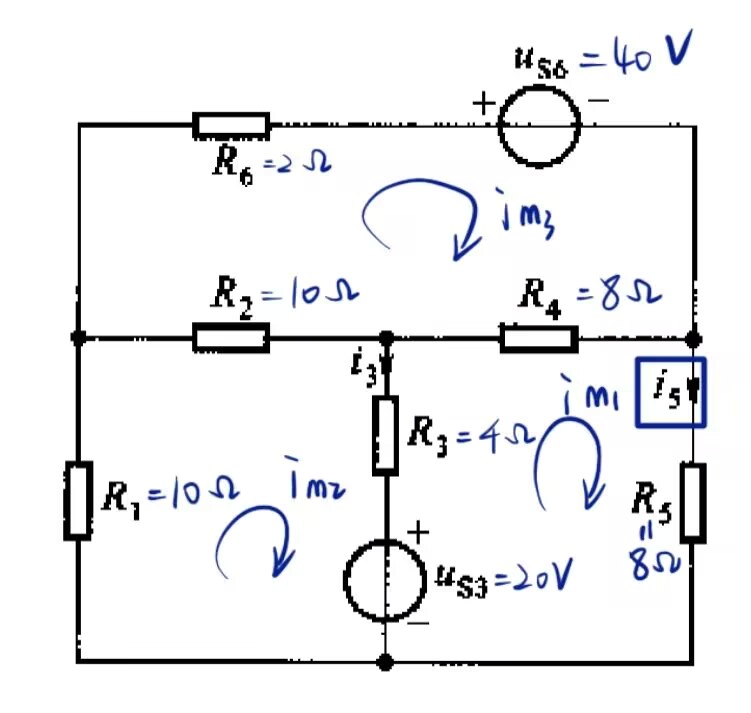
\includegraphics[width=0.4\textwidth,height=0.2\textheight]{3-8.jpg}
\end{center}

解:
\[
\begin{bmatrix}
    20&-4&-8\\
    -4&24&-10\\
    -8&-10&20
\end{bmatrix}
\begin{bmatrix}
    i_{m1}\\
    i_{m2}\\
    i_{m3}
\end{bmatrix}
=\begin{bmatrix}
    20\\
    -20\\
    -40
\end{bmatrix}
\Rightarrow
\begin{bmatrix}
    i_{m1}\\
    i_{m2}\\
    i_{m3}
\end{bmatrix}
=\begin{bmatrix}
    -0.956\\
    -2.507\\
    -3.636
\end{bmatrix}
\]
故$i_5=i_{m1}=-0.956A$.
\section*{3-21}
用节点电压法求图中电压$U$
\begin{center}
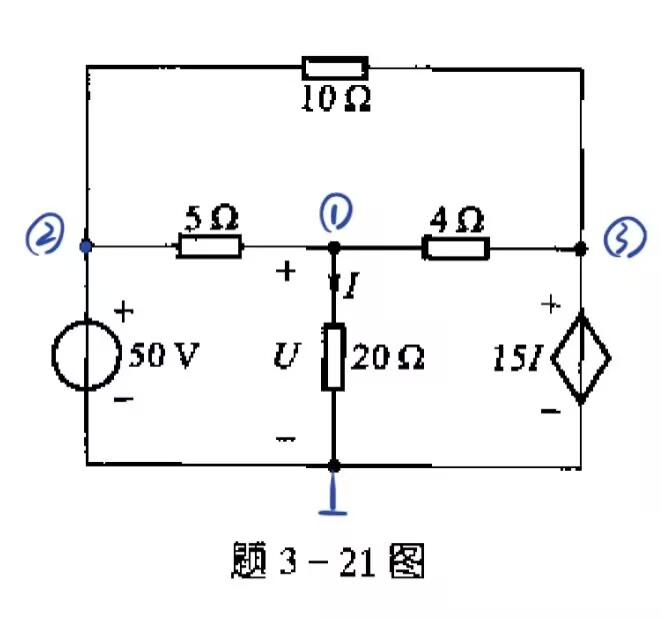
\includegraphics[width=0.4\textwidth,height=0.2\textheight]{3-21.jpg}
\end{center}

解:$u_{n2}=50V$,$u_{n3}=15I$,且有$I=0.05u_{n1}$

对节点1:
\[0.5u_{n_1}-0.2u_{n_2}-0.25u_{n_3}=0\]\[
\Rightarrow U=u_{n_1}=20.3V
\]
\section*{3-22}
用节点电压法求图(a)中的$U_x$和图(b)中的$I$
\begin{center}
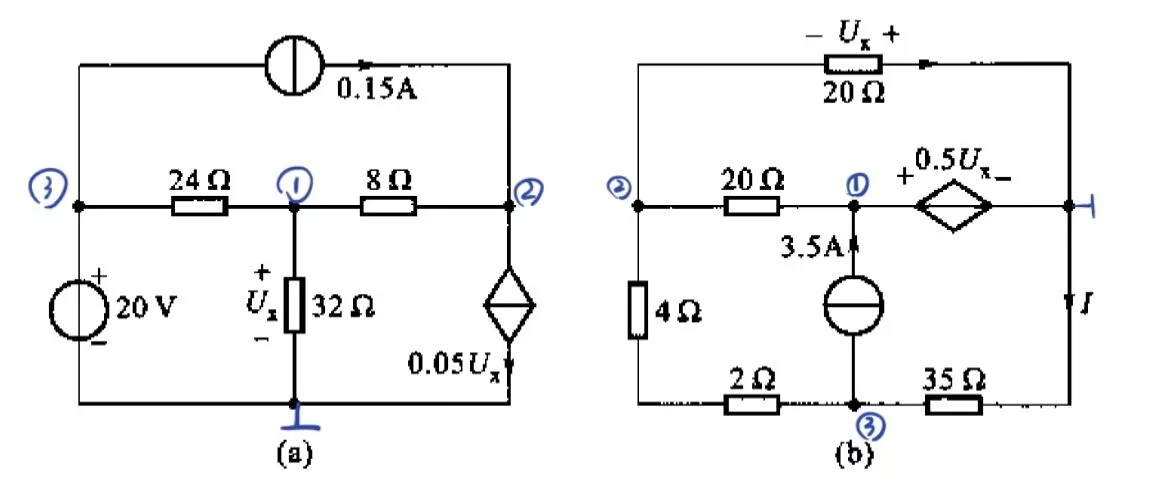
\includegraphics[width=0.8\textwidth,height=0.2\textheight]{3-22.jpg}
\end{center}

(a)解:$u_{n2}=30V$,$u_{n1}=U_x$

对Node1:
\[(\frac{1}{24}+\frac{1}{8}+\frac{1}{32})u_{n1}-
\frac{1}{8}u_{n2}-\frac{1}{24}u_{n3}=0\]

对Node2:
\[
\frac{1}{8}u_{n_2}-\frac{1}{8}u_{n1}=0.15-0.05U_x
\]

解得:
\[U_x=8V\]

(b)解:$u_{n1}=0.5U_x$,$u_{n2}=-U_x$
\[\begin{cases}
    (\frac{1}{6}+\frac{1}{35})u_{n3}-\frac{1}{6}u_{n2}=-3.5\\
    (\frac{1}{6}+\frac{1}{20}+\frac{1}{20})u_{n2}-\frac{1}{20}u_{n1}-\frac{1}{6}u_{n3}=0
\end{cases}\]
\[\Rightarrow
I=1A\]
\section*{3-23}
用节点电压法求图中电路$I_x$以及ccvs的功率
\begin{center}
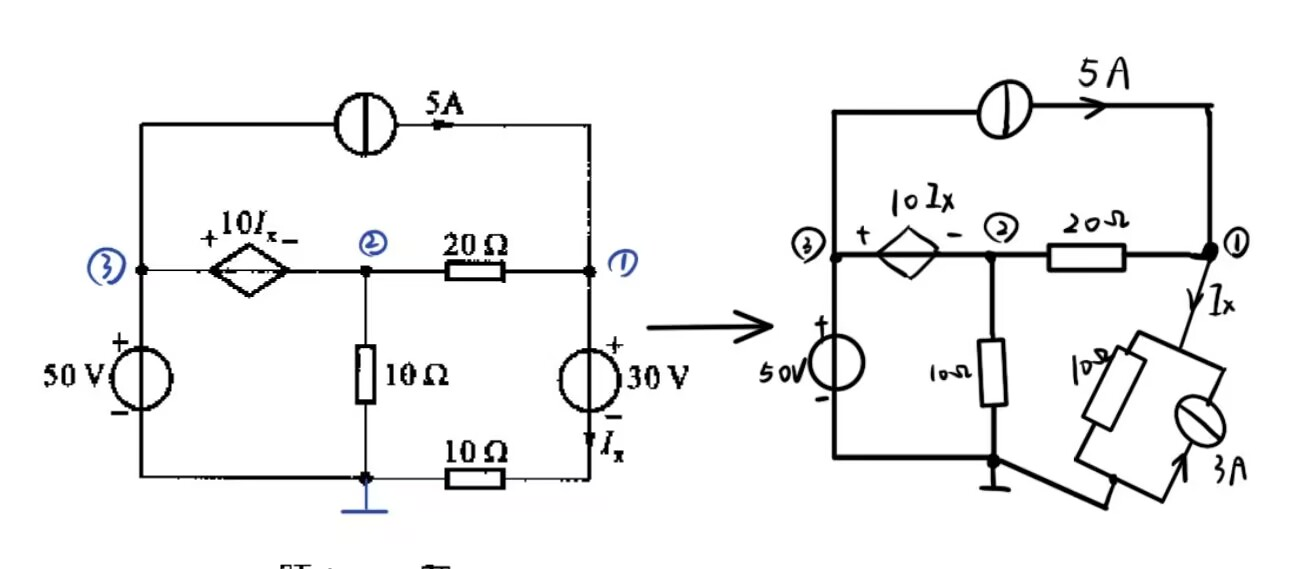
\includegraphics[width=0.8\textwidth,height=0.2\textheight]{3-23.jpg}
\end{center}

解:
$u_{n3}=50V$,$u_{n2}=50-10I_x$

node1:
\[
(\frac{1}{20}+\frac{1}{10})u_{n1}-\frac{1}{20}u_{n2}=5+3
\]

另有:
\[
\frac{u_{n1}}{10}-3=I_x
\]
\[
\Rightarrow I_x=3A\text{,}u_{n1}=60V
\]

于是$u_{n2}=20V$,对node 2用KCL:
\[
\frac{60V-20V}{20\Omega}=\frac{20V}{10\Omega}+I_{CCVS}
\]
\[\Rightarrow I_{CCVS}=0\Rightarrow P_{CCVS}=0
\]
\end{document}